%! Author = giaco
%! Date = 16/05/2024

\chapter{Method}
\label{sec:method}
The focus of this work is to simplify as much as possible the representation learning of current RL algorithms leveraging prior knowledge and letting the agent focus on learning the actual policy to solve the task.
Many previous work already, mentioned in Sec. \ref{sec:fm_rl}, share the idea of leveraging FMs to enhance the state representation facilitating the transfer of the world knowledge and simplifying the RL training process.
Differently from these studies, our methodology is designed to enhance the efficiency and effectiveness of RL agents by leveraging a set of pre-trained models tailored to the current task.
First, our work proposes a set of basic abilities like humans have.
RL agents are equipped with these FMs, which serve as the prior knowledge needed to generate diverse representations of the environment.
FMs weights are frozen during the training process.
Then, we focus on how to effectively combine their latent representations to improve agents performance.

While agents interact with the environment, the current observation is collected and processed through each pre-trained models.
This process yields multiple perspectives or views of the world, each encoded uniquely based on the specific model.
These features represent different facets of the environment, providing the agent with a comprehensive and enhanced understanding of the current state.
The challenge then lies in integrating these disparate views into a cohesive and enriched representation.
To achieve this, we employ a specialized combination module, that synthesizes the information from the various models into a single latent representation.
The intuition is that the enriched representation provides a comprehensive understanding of the current state of the environment, derived from the collective insights of the pre-trained models.
By leveraging FMs, our approach significantly reduces the burden on the RL agent to learn the environmental representation from scratch, allowing it to focus more on refining the action-mapping process.
This not only accelerates the learning process but also enhances overall performance by providing a well-structured and informative representation.

The architecture of our agents is divided into two main components.
The first part takes care of processing the current observation into multiple latent representations and then combines them into a single enriched representation.
We refer to this part as the \textit{Feature Extractor} module.
Feature extractor part is in turn divided into two sub-modules, the first compute the preprocessing of the information through the FMs, the latter is the combination module that merges the representations.
Finally, the second part is the policy learning network, where the unified representation is fed into a small neural network whose responsibility is to map the latent encoding to actions.

In the following sections, we will describe in detail the different combination modules that we adopted to merge the representations extracted by the FMs.
First we focus on the \textit{Weight Sharing Attention} module, which is the module that we propose as a solution to the problem of combining different FMs, and we think that it deserves more relevance.
Then, we will briefly describe other combination modules that we tested to compare the performance of the agents.

\section{Weight Sharing Attention}
\label{sec:wsa}
With a view to lifelong learning agents, the aim is therefore to equip the agent with prior skills that can be changed or improved over time to adapt to new unseen tasks.
To this end, a model capable of re-adapting to new abilities with little or no effort is needed.
To facilitate the integration of different pre-trained models, we propose WSA\@.
The WSA module leverages the concept of \textbf{weight sharing}, as seen for the first time in CNNs~\citep{fukushima1980neocognitron}, and attention~\citep{vaswani2017attention} principles to efficiently merge outputs from diverse FMs.

%maybe change
In specific, WSA dynamically adjusts the weights assigned to each pre-trained model based on the current context, emphasizing the most relevant models for the current state.

Supposing to have a set of $k$ pre-trained models $\Psi = \{\psi_1, \psi_2, \ldots, \psi_k\}$, each model $\psi_i$ is used to extract features from the current observation $\mathcal{O}$.
Each pre-trained model is equipped with an adapter $\mathcal{A}$, which is a small neural network consisting of a linear layer followed by a non-linearity layer, in this case a ReLU activation function.
The adapter is used to resize the latent representation of the pre-trained model to a fixed size, ensuring compatibility among different models.
As a result of this operation, each FM outputs an embedding $E_i$ of a predefined size.
The weights of the adapters are optimized during training.

Among the provided FMs, one model is used as State Encoder $\mathcal{E}$ to compute a representation of the current state, which serves as \textit{context} $\mathcal{C}$ for the attention mechanism.
Also for this model, the same kind of adapter is used to resize the latent representation to the same fixed size.


To compute the attention weights, we use a shared MLP $f_\theta$ that takes as input the context $\mathcal{C}$ concatenated with the single embedding $E_i$ of each FM\@.
This MLP outputs the model-specific weight $w_i$ to determine the contribution of each model in the final representation.
It is important to note that this MLP is shared across all models, ensuring uniform weight computation.
By dynamically adjusting weights based on the current context, WSA emphasizes the most relevant models for any given situation, resulting in a more accurate and adaptable representation.
The final representation $\mathcal{R}$ is computed using the weights for all pre-trained models and computing a weighted sum of their embeddings.
The output obtained is so a combination of the various perspectives, provided by the pre-trained models, into a single enriched latent representation.
This final representation is used for action mapping, enhancing the performance and learning efficiency of RL agents by integrating the strengths of multiple FMs.


The approach by design guarantees two additional features.
WSA adds \textbf{explainability} to the model.
By examining the weights assigned to different pre-trained models, we can gain insights into which models are most influential in a given context.
This achieves a more transparent decision-making process of RL agents.
Additionally, WSA is \textbf{scalable} and \textbf{adaptable} to any number of pre-trained models.
Its shared component can handle an arbitrary number of models, making it a flexible solution for dynamically evolving agents.


Figure~\ref{fig:main_architecture} shows the main architecture of our agent, with an emphasis on the WSA module.
Algorithm~\ref{alg:wsa} instead reports the pseudocode for the actual implementation.

\begin{algorithm}[ht]
    \caption{Weight Sharing Attention}\label{alg:wsa}
    \texttt{In \textcolor{blue}{blue} we highlight the components that are updated during training.}\\
    \begin{algorithmic}[1]
        \Require Current observation $\mathcal{O}$, List of FMs $\Psi$, State Encoder $\mathcal{E}$
        \State $\mathcal{C} = \textcolor{blue}{\mathcal{A}_0}(\mathcal{E}(\mathcal{O}))$ \Comment{Compute current context representation}
        \For {FM $\psi$ in $\Psi$}
            \State $x = \psi_i(\mathcal{O})$ \Comment{Forward pass using current state}
            \State $E_i = \textcolor{blue}{\mathcal{A}_i}(x)$ \Comment{Use the adapters to compute the resized embedding}
            \State $w_i = \textcolor{blue}{f_\theta}(\mathcal{C}, E_i)$ \Comment{Compute the weight for current model using shared component}
        \EndFor
        \State $\mathcal{R} = \sum_{i=0}^{|\Psi|} w_i * E_i$ \Comment{Final representation: weights $W$, embeddings $E$ $\rightarrow$ $W \cdot E$}
    \end{algorithmic}
\end{algorithm}



\begin{figure}[ht]
    \begin{center}
        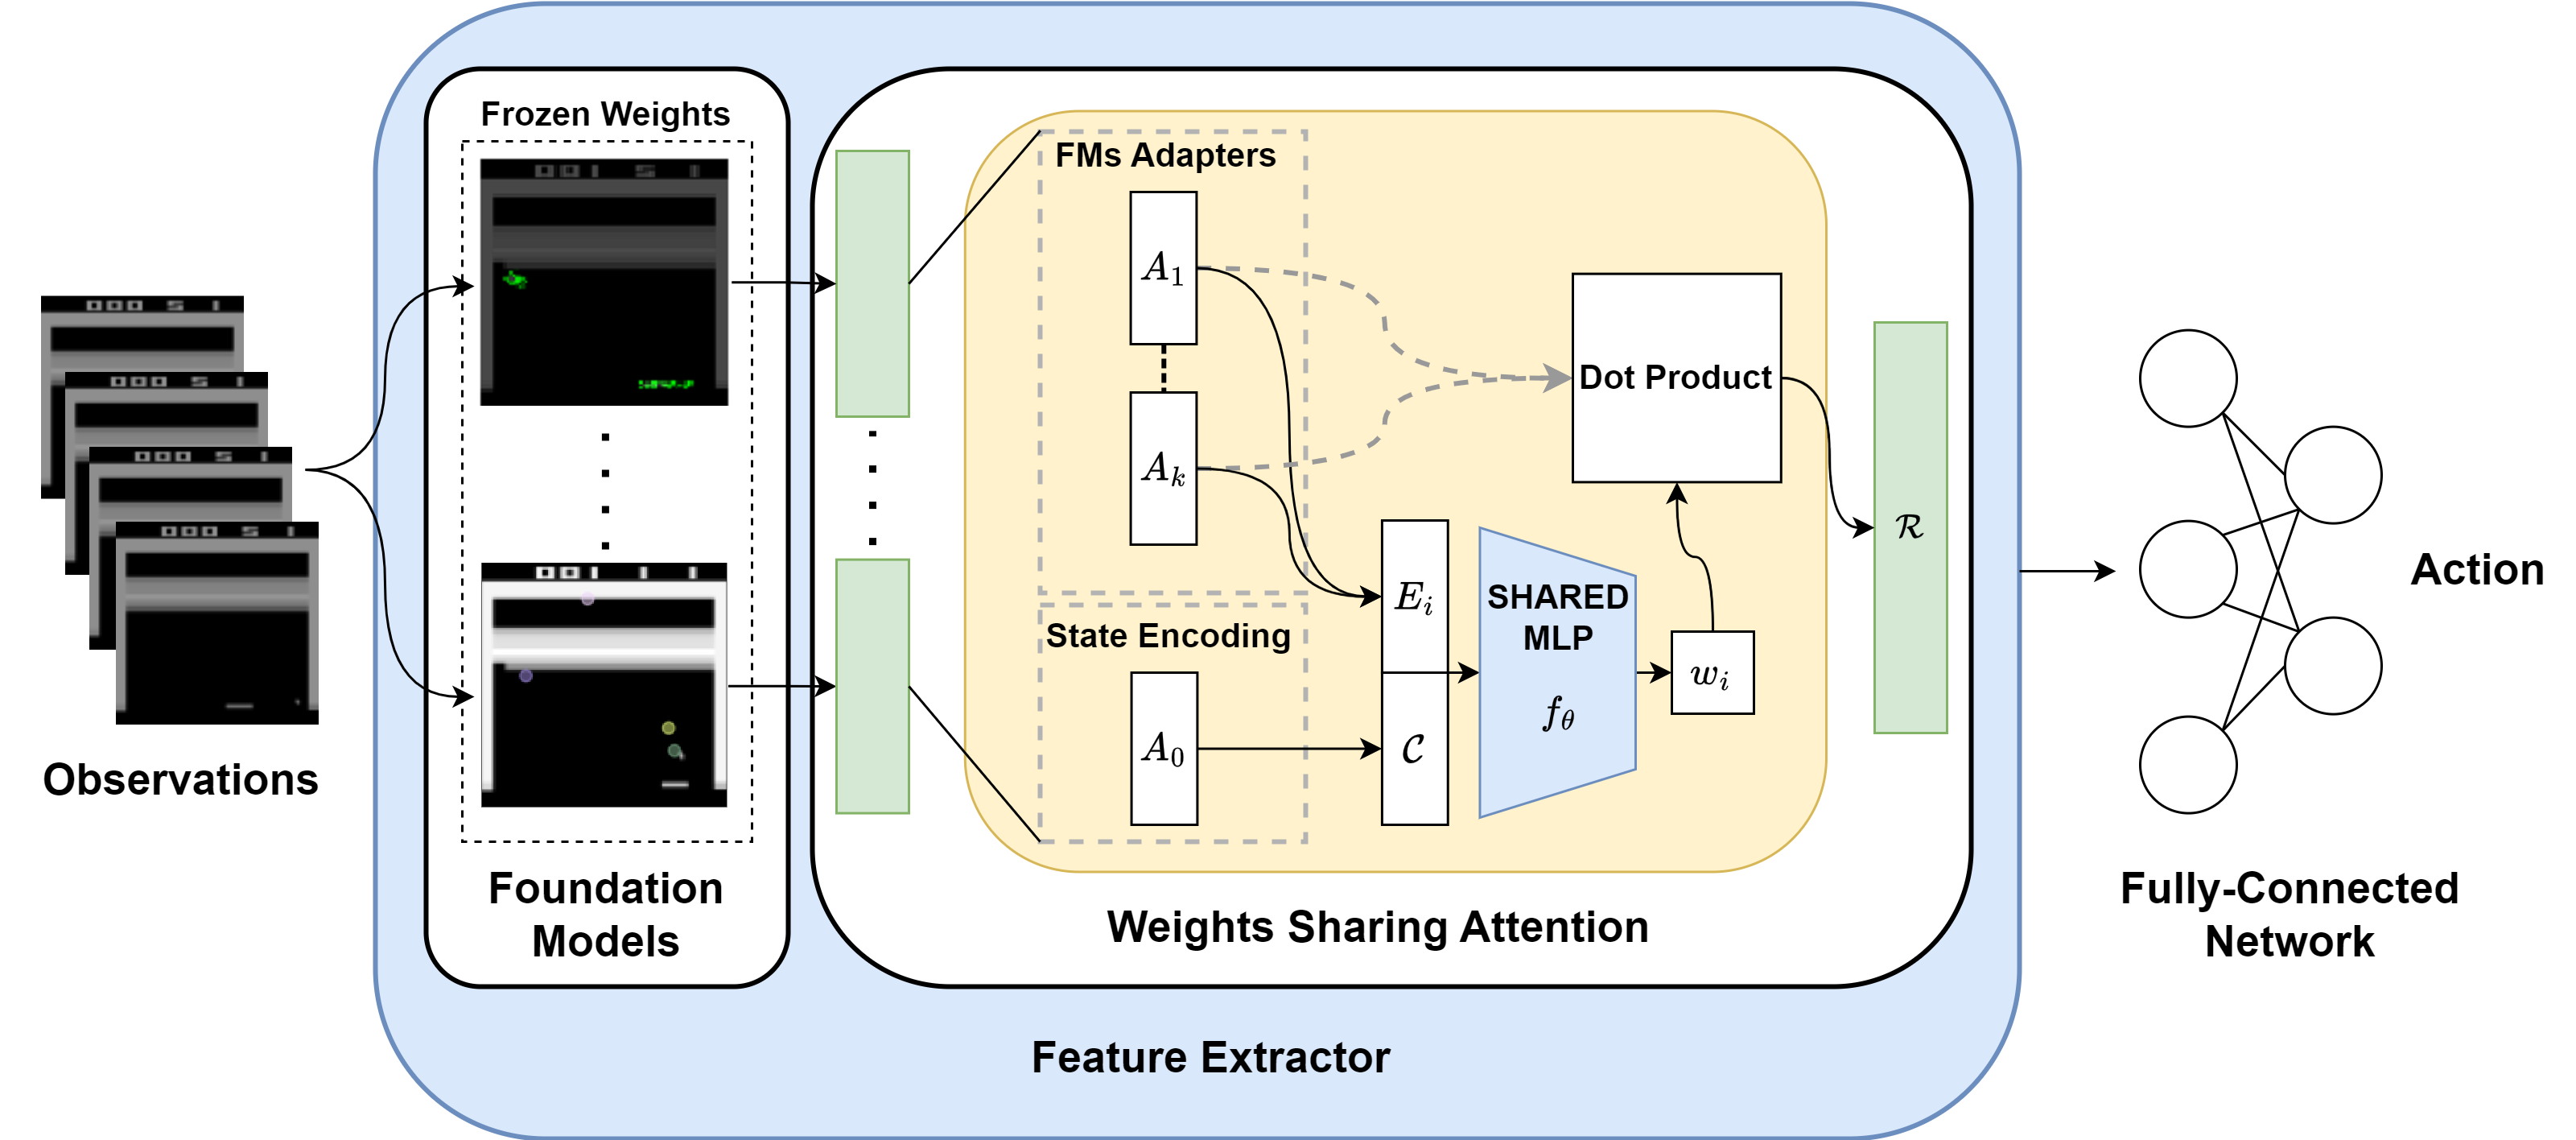
\includegraphics[width=1\textwidth]{images/main_architecture2}
    \end{center}
    \caption{A schematic representation of the main pipeline from observation to actions and WSA architecture. The last four frames are stacked together and passed as input to the FMs and their adapters $\mathcal{A}_1, \dots \mathcal{A}_k$ to obtain an embedding of the current state. A State Encoder $\mathcal{E}$ and its adapter $\mathcal{A}_0$ compute an encoding of the state, that will be used as context $\mathcal{C}$. A shared MLP layer takes as input the context $\mathcal{C}$ and the representation of the $i^{th}$ FM, $E_i$, and predicts the weight for that specific model. The final enriched representation $\mathcal{R}$ is obtained from the weighted summation between each weight $w_i$ and its respective embedding $E_i$. $\mathcal{R}$ is given as input to agents' \texttt{Fully-Connected Network}.}
    \label{fig:main_architecture}
\end{figure}









% Although very significant, the skills defined up to this point may not provide enough information for the agent to learn. Therefore, we decided to enrich our skill set by using the well-known model based on convolutional layers specified in \cite{mnih2013playing}, which we refer to as \textit{Nature CNN}, as a base architecture to develop other simple skills.
% In fact, Nature CNN has been used in various forms of encoder-decoder to implement: 1) an Autoencoder that takes the last frame of a game, encodes it in a latent space, and then tries to reconstruct the original frame; 2) an Image Completion model that given a frame of a game that is occluded with a black square, tries to reconstruct the original frame without occlusion; 3) finally a Frame Prediction model that given the last four frames of a game, tries to predict and reconstruct the frame 5 steps ahead.
% These last three models were all trained with grayscale game frames of size 84x84 pixels. For the Frame Prediction model, on the other hand, we thought that predicting the frame at the next step might not be very informative since the frame would be very similar to the current one, so we decided to try to predict the frame 5 steps ahead.

%inserire qualche frase in più su come abbiamo create queste ultime 3 skill?, sul perchè abbiamo scelto questi modelli, sul fatto che non soon perfetti in quanto molte volte non predicono bene l'output ma che comunque possono codificare informazioni important per l'agente

% The architecture of Nature CNN has been slightly modified as it appears in Tab. \ref{tab:nature_cnn} to match the output dimensions of the other skills so that they can be properly concatenated.


%spiegare un po meglio questa parte, non abbiamo un modello generic ma alleniamo una singola skill per ogni ambient al contrario di SIMA
% Finally, all of these models are not general. We decided to specialize the skills by creating a model for each skill and environment.

% \begin{table}[htbp]
%     \begin{center}
%         \begin{tabular}{lllll}
%             \multicolumn{1}{l}{LAYER}  &\multicolumn{1}{l}{\bf IN. CHANNELS}  &\multicolumn{1}{l}{\bf OUT CHANNELS}  &\multicolumn{1}{l}{\bf KERNEL SIZE}  &\multicolumn{1}{l}{\bf STRIDE}
%             \\ \hline \\
%             1st CNN Layer   &  1 or 4  & 32 & 8 & 4 \\
%             2nd CNN Layer   &  32  & 64 & 3 & 1 \\
%             3rd CNN Layer   &  64  & 64 & 3 & 1 \\

%         \end{tabular}
%     \end{center}
%     \caption{This table shows the encoder architecture of Autoencoder, Image Completion, and Frame Prediction models. Input channels for the first convolutional layer are 1 or 4 depending on the model. Autoencoder and Image Completion take as input 1 frame in grayscale while Frame Prediction takes as input the last 4 grayscale frames stacked along the channel dimension. The stride on the second convolutional layer was decreased from 2 to 1 with respect to Nature CNN to match the output dimensions of other skills. Each convolutional layer is followed by a ReLU activation function. The decoder part is specular.}
%     \label{tab:nature_cnn}
% \end{table}










%starting from the FMs used to extract information from the environment, then moving to the combination modules used to merge the different representations, and finally, we will describe the policy learning network.

%the second part

%as shown in Figure~\ref{fig:main_architecture}.
%The first one, delimited by the \textcolor{blue}{blue} box, handles the processing of the current observation into a latent representation.
%\textcolor{orange}{yellow} box,






























\section{Other Combination Modules}
\label{sec:combination_modules}
% Knowledge Skills are concatenated together in order to solve complex tasks that require a composition of different state representations.
% Assuming we have \textit{k} different skills, each of which can extract features in different spaces e.g. linear skills that produce an embedding or skills that work in the spatial field and output a set of feature maps, we have tried different ways of concatenating the skills, which we will list below one after the other.

% \textbf{Linear Concatenation Extractor}
% This way of concatenating skills is the simplest. Skills that output a one-dimensional vector are left as they are. Skills that operate in the spatial field are flattened to produce a one-dimensional vector.
% The embeddings of each skill are concatenated to create a large feature vector. This feature vector is given as input to the policy learning network.

% \textbf{Fixed Linear Concatenation Extractor}
% One problem with the linear concatenation extractor is that the skills may have very different dimensionality. One skill might become much more important than the others just because its dimension is larger than the others. So, considering that we have \textit{k} different skills, after obtaining a linear representation as in the previous extractor for each one, we mapped that representation into an embedding of fixed dimensions using \textit{k} different linear layers with the same size.
% The new embeddings are then concatenated as before and used as input for the rest of the network.

% \textbf{CNN Concatenation Extractor}
% As mentioned earlier, skills operate in different spaces. In this case, the skills operating in the linear field are reshaped to match the dimensions in the spatial field of the other skills.
% The skills are then concatenated along the channel dimension and passed to one or more convolutional layers to extract features.
% At this point, the output of the convolutional layer is flattened and the embedding is passed to the rest of the network.

% \textbf{Combine Extractor}
% This way of concatenating skills is a mixture of the previous ones. In this case, first of all, the skills operating in the spatial field are concatenated with each other along the channel dimension and passed through a convolutional layer. Then they are flattened and the resulting embedding is concatenated to the linear skills.

% \textbf{Reservoir Concatenation Extractor}
% With this way of concatenating, we decided to explore reservoir dynamics properties to map the input into a lower-dimension latent space using a non-linear transformation.
% So, first of all, we created a large embedding concatenating the skills as in the Linear Concatenation, and then we used this vector as input for the reservoir obtaining as output a vector of the size of the reservoir. This new state representation is used as input to the policy learning network.

% \textbf{Dot Product Attention Extractor}
% Another possible solution is to combine representations using attention-like mechanisms conditioned on the configuration of the environment.
% The idea is to understand which skills are useful and worth being included in the final representation given the current state. Some skills might be more important in some
% specific set of states than others, moreover, this approach would help to implicitly add explainability to the model.
% For this purpose, we used the \textit{scaled dot product attention} \cite{vaswani2017attention}.
% %implemented in a module currently available in beta on PyTorch.
% %inserire il riferimento al link? https://pytorch.org/docs/stable/generated/torch.nn.functional.scaled_dot_product_attention.html
% As with the Fixed Linear Concatenation Extractor, the skill representations are reduced to a vector of fixed size. These, however, are stacked together to form a tensor of shape \textit{(number\_of\_skills * vector\_size)}. This constitutes the \textbf{key} part and the \textbf{value} part of the attention module.
% For the \textbf{query} part, we used the Autoencoder model defined in \ref{sec:skills} to encode the current state of the game in a latent space. We then used a linear layer of the same dimensions as the one used for the skills in order to obtain a vector of the same dimensions. This therefore represents the context.
% The output of the attention module is the weighted sum of skill embeddings considering the context, it will then be passed as input to the rest of the network for policy learning.

% \textbf{Weights Sharing Attention Extractor}
% Intending to have a set of skills that can be interchanged in the future, it is necessary to have a model that can be easily adapted to unseen new skills and that is easy to re-train.
% To this end, we call \textit{Weights Sharing Attention} an attention-like mechanism such that given a linear layer to which we input the embedding of a skill $s_i$ concatenated with the embedding of a context \textit{c}, it outputs a scalar value representing the weight $w_i$ of that skill considering the context. The weighted sum of all the skills embeddings for their weight is then computed. The resulting vector will be passed to the rest of the network.
% Since we think that this method is not straightforward in Fig. \ref{fig:wsharingmodule}  we will show the architecture.

% \begin{figure}[ht]
%     \begin{center}
%         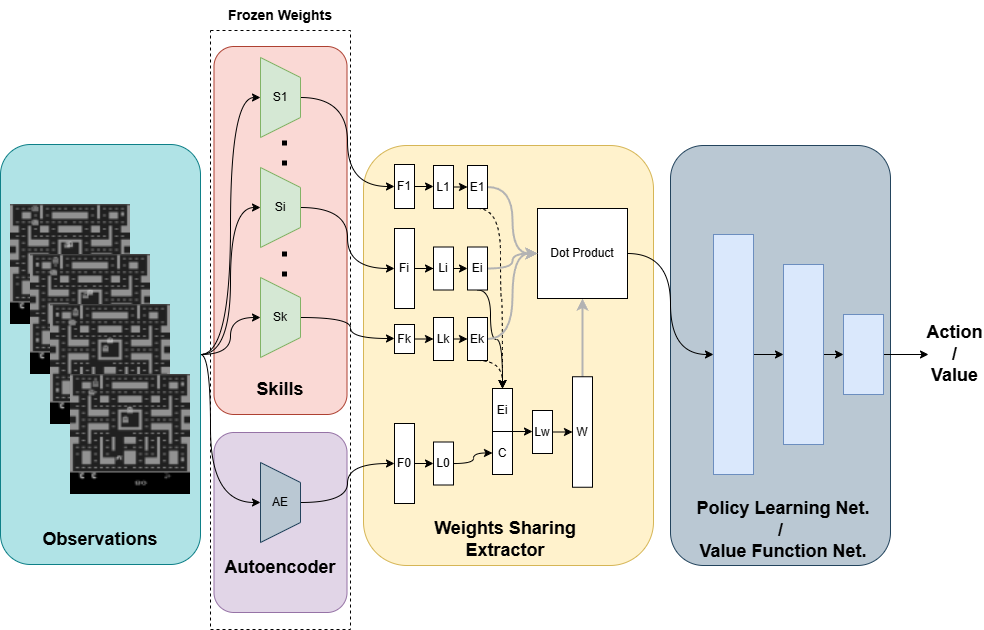
\includegraphics[width=\textwidth]{images/wsharing_module.png}
%     \end{center}
%     \caption{In Figure we show the Weights Sharing Attention Module. Each skill embedding $F_i$ is given as input to a different linear layer $L_i$. This is done to learn a representation of the skills and fix the size of the embeddings so that they are all equal. The same process is done for the autoencoder output so that the embedding for the context \textit{c} is created. At this point, for each skill, the context vector is concatenated with the embedding $E_i$ of a skill defining the input for the linear layer $L_w$ that will return the weight for the specific skill $w_i$, thus constituting the vector of weights \textbf{W}. Finally, the weighted sum $w_1*E_1 + w_2*E_2 + .... + w_k*E_k$ will be the new state representation to be passed to the agent. Each linear layer is followed by a ReLU layer.}
%     \label{fig:wsharingmodule}
% \end{figure}